\documentclass[aspectratio=169, 9pt, handout]{beamer}\usepackage[]{graphicx}\usepackage[]{color}
% maxwidth is the original width if it is less than linewidth
% otherwise use linewidth (to make sure the graphics do not exceed the margin)
\makeatletter
\def\maxwidth{ %
  \ifdim\Gin@nat@width>\linewidth
    \linewidth
  \else
    \Gin@nat@width
  \fi
}
\makeatother

\definecolor{fgcolor}{rgb}{0.345, 0.345, 0.345}
\newcommand{\hlnum}[1]{\textcolor[rgb]{0.686,0.059,0.569}{#1}}%
\newcommand{\hlstr}[1]{\textcolor[rgb]{0.192,0.494,0.8}{#1}}%
\newcommand{\hlcom}[1]{\textcolor[rgb]{0.678,0.584,0.686}{\textit{#1}}}%
\newcommand{\hlopt}[1]{\textcolor[rgb]{0,0,0}{#1}}%
\newcommand{\hlstd}[1]{\textcolor[rgb]{0.345,0.345,0.345}{#1}}%
\newcommand{\hlkwa}[1]{\textcolor[rgb]{0.161,0.373,0.58}{\textbf{#1}}}%
\newcommand{\hlkwb}[1]{\textcolor[rgb]{0.69,0.353,0.396}{#1}}%
\newcommand{\hlkwc}[1]{\textcolor[rgb]{0.333,0.667,0.333}{#1}}%
\newcommand{\hlkwd}[1]{\textcolor[rgb]{0.737,0.353,0.396}{\textbf{#1}}}%
\let\hlipl\hlkwb

\usepackage{framed}
\makeatletter
\newenvironment{kframe}{%
 \def\at@end@of@kframe{}%
 \ifinner\ifhmode%
  \def\at@end@of@kframe{\end{minipage}}%
  \begin{minipage}{\columnwidth}%
 \fi\fi%
 \def\FrameCommand##1{\hskip\@totalleftmargin \hskip-\fboxsep
 \colorbox{shadecolor}{##1}\hskip-\fboxsep
     % There is no \\@totalrightmargin, so:
     \hskip-\linewidth \hskip-\@totalleftmargin \hskip\columnwidth}%
 \MakeFramed {\advance\hsize-\width
   \@totalleftmargin\z@ \linewidth\hsize
   \@setminipage}}%
 {\par\unskip\endMakeFramed%
 \at@end@of@kframe}
\makeatother

\definecolor{shadecolor}{rgb}{.97, .97, .97}
\definecolor{messagecolor}{rgb}{0, 0, 0}
\definecolor{warningcolor}{rgb}{1, 0, 1}
\definecolor{errorcolor}{rgb}{1, 0, 0}
\newenvironment{knitrout}{}{} % an empty environment to be redefined in TeX

\usepackage{alltt}

% \transdissolve[duration=0.2] % Only works with Adobe Acrobat

% Some important packages
\usepackage{apacite}
\usepackage{epstopdf}
\hypersetup{colorlinks=false, allcolors=purple}
\usepackage{booktabs}
\linespread{1.3}
\usepackage{tabularx}
% \usepackage{textpos}  % for the textblock* environment
\usepackage{geometry}
\usepackage{algorithm2e}
\usepackage{amsmath, amssymb}

\usepackage{natbib}
\renewcommand{\bibsection}{\subsubsection*{\bibname } }


% Styles
\usepackage{xcolor}
\definecolor{suffstat}{RGB}{10,159,0}
\definecolor{normconst}{RGB}{87,38,231}

% Noice!
\usetheme{usckeck}

\title[Stat. Comp. Bioinf \& SocNets.]{Statistical and computational methods for bioinformatics and social network analysis\linebreak{\small or how did I learn to stop worrying and love the bomb}}
\author[GGVY]{George G Vega Yon}
\institute[USC-PREVMED]{University of Southern California, Department of Preventive Medicine}

% Some definitions
\def\cursection{\frame{\frametitle{Contents}\tableofcontents[current]}}
\newcommand{\ergmitopkg}[0]{\texttt{ergmito}}
\newcommand{\aphylopkg}[0]{\texttt{aphylo}}
\graphicspath{{.}{fig/}}


% ------------------------------------------------------------------------------
% ------------------------------------------------------------------------------
% --------------------------- END OF PREAMBLE ----------------------------------
% ------------------------------------------------------------------------------
% ------------------------------------------------------------------------------
\IfFileExists{upquote.sty}{\usepackage{upquote}}{}
\begin{document}
% \SweaveOpts{concordance=TRUE}

% ------------------------------------------------------------------------------
\begin{frame}[noframenumbering]
\maketitle
\end{frame}

% ------------------------------------------------------------------------------
\begin{frame}
\frametitle{Motivation}

\begin{center}
\large
\textcolor{usccardinal}{\bf Statistical and computational methods for\\ %
bioinformatics and social network analysis}
\end{center}

\begin{itemize}
\item We live in a non-{\it IID} world.
\item Some times, looking the whole helps understanding the parts.
\item We have the computational tools to do such.
\end{itemize}
\end{frame}

% ------------------------------------------------------------------------------
\section{Paper 1: Exponential Random Graph Models for Small Networks}
\frame{\frametitle{Contents}\tableofcontents}
\cursection

% \frame{\sectionpage}

\begin{frame}
\frametitle{What are Exponential Random Graph Models}

Exponential Family Random Graph Models, aka \alert{ERGMs} are:\pause

\begin{itemize}[<+->]
\item Statistical models of (social) networks
\item In simple terms: statistical inference on what network patterns/structures/motifs
govern the data-generating process
\begin{figure}
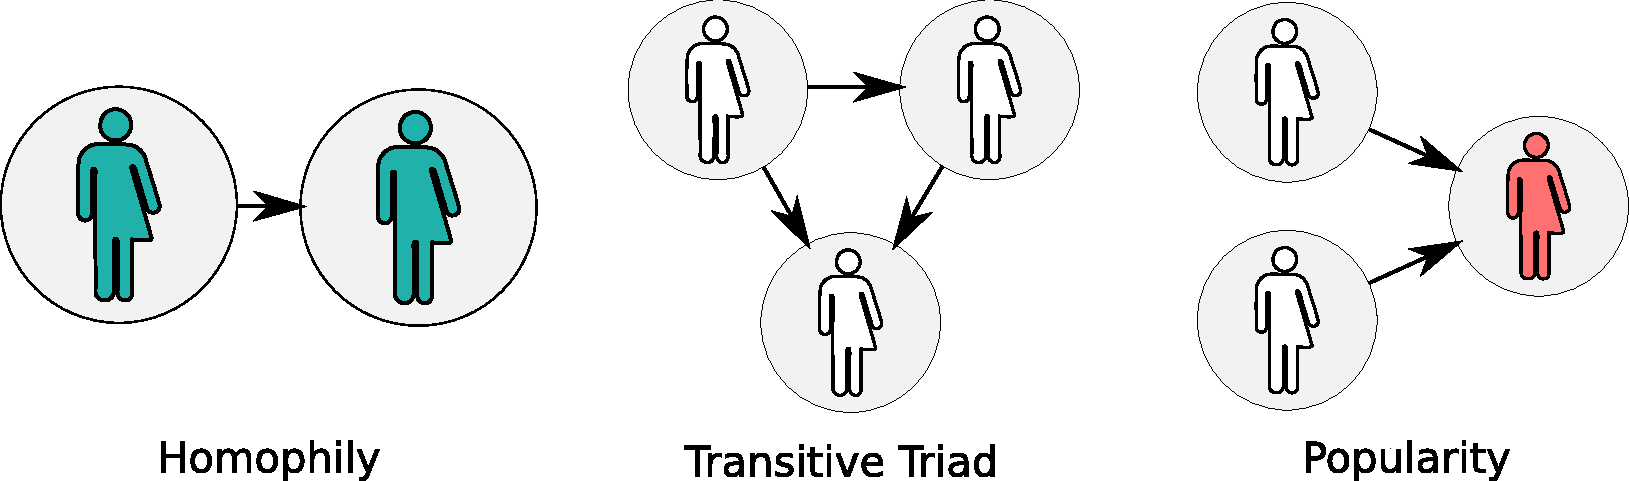
\includegraphics[width=.6\linewidth]{friendly-terms.pdf}
\end{figure}
\end{itemize}

\end{frame}

% ------------------------------------------------------------------------------
\begin{frame}[label=ergmeq]
\frametitle{ERGMs (cont'd)}
\begin{figure}
\centering
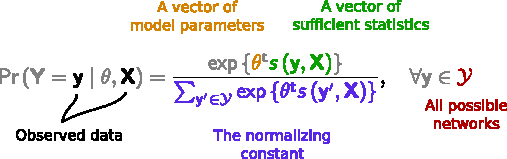
\includegraphics[width=.7\linewidth]{parts-of-ergm.pdf}
\end{figure}

\uncover<2->{The normalizing constant has $2^{n(n-1)}$ terms!}

\vfill\hfill \hyperlink{ergmterms}{\beamergotobutton{more on terms}}
\end{frame}


% ------------------------------------------------------------------------------
\begin{frame}[label=art]
\frametitle{ERGMs: State of the Art}
\pause
Medium-large (dozens to a couple of thousand vertices) networks

\begin{itemize}
\item Markov Chain Monte Carlo (MCMC) based approaches like MC-MLE or Robbins-Monro Stochastic Approximation. \hyperlink{mcmle}{\beamergotobutton{details}}
\item Maximum Pseudo Likelihood (MPLE)
\end{itemize}\pause

large-huge networks (up to the millions of vertices)

\begin{itemize}
\item Semi-parametric bootstrap
\item Conditional joint estimation (like snowball sampling, a.k.a. divide and conquer)
\item Equilibrium Expectation Algorithm (millions of vertices)
\end{itemize}\pause

What about small networks?

\end{frame}

% 
% % ------------------------------------------------------------------------------
% \begin{frame}
% \frametitle{Do we care about small networks?}
% \begin{figure}
% \centering
% 
\includegraphics[width=.6\linewidth]{american-chopper-argument-ergmitos.png}
% \end{figure}
% \end{frame}

% ------------------------------------------------------------------------------
\begin{frame}
\frametitle{Do we care about small networks?}

\begin{minipage}{.40\linewidth}
We see small networks everywhere\pause

\begin{itemize}[<+->]
\item Families and friends
\item Small teams
\item Egocentric networks
\item Online networks (sometimes)
\item etc.
\end{itemize}
\end{minipage}\pause
\hfill
\begin{minipage}{.55\linewidth}

\includegraphics[width=.95\linewidth]{american-chopper-argument-ergmitos.png}
\end{minipage}

\end{frame}

% ------------------------------------------------------------------------------
\begin{frame}
\frametitle{ERGMs for small networks}

From the methodological point of view, current methods are great, but:\pause

\begin{itemize}
\item Possible accuracy issues (error rates)\pause
\item Prone to degeneracy problems (sampling and existance of MLE)\pause
\item It is not MLE...
\end{itemize}

\end{frame}

% ------------------------------------------------------------------------------
\begin{frame}[label=ergmito]
\frametitle{ERGMs for Small Networks}

\pause
\begin{itemize}[<+->]

\item In the case of small-enough networks, computation of the likelihood becomes
computationally feasible.

\item For example, a network with 5 nodes has 1,048,576
unique configurations.

\item This allow us to directly compute {\bf\color{normconst} the normalizing constant}.

\item Using the exact likelihood opens a huge window of methodological-possibilities.

\item We implemented this and more in the \ergmitopkg{} R package \hyperlink{ergmitopkg}{\beamergotobutton{more}}

\end{itemize}




\end{frame}

% ------------------------------------------------------------------------------
\begin{frame}[label = ergmitoexample]
\frametitle{\ergmitopkg{} example}

\begin{minipage}{.4\linewidth}
\begin{figure}
\centering
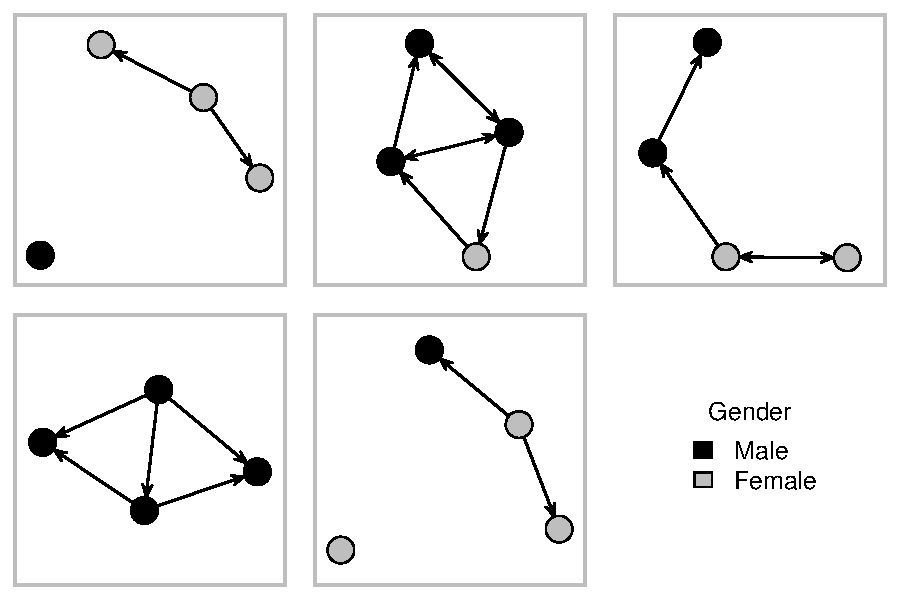
\includegraphics[width = .9\linewidth]{fivenets_graphs.pdf}
\caption{Random sample of 5 networks simulated using the ergmito package}
\end{figure}
\end{minipage}
\hfill
\begin{minipage}{.55\linewidth}
\pause
\footnotesize
\begin{table}
\begin{tabular}{l*{2}{m{.2\linewidth}<\centering}}
\hline
 & Edgecount & Full model \\
\hline
Edgecount             & $-0.69^{*}$ & $-1.70^{**}$ \\
                      & $(0.27)$    & $(0.54)$     \\
Homophily (on Gender) & & $1.59^{*}$   \\
                      & & $(0.64)$     \\
\hline
AIC                   & 78.38       & 73.34        \\
BIC                   & 80.48       & 77.53        \\
Log Likelihood        & -38.19      & -34.67       \\
Num. networks         & 5           & 5            \\
\hline
\multicolumn{3}{l}{\scriptsize{Standard errors in parenthesis. $^{***}p<0.001$, $^{**}p<0.01$, $^*p<0.05$}}
\end{tabular}
\caption{Fitted ERGMitos using the fivenets dataset.}
\label{table:coefficients}
\end{table}
\normalsize
\end{minipage}\pause

We performed a large simulation study \hyperlink{ergmitodgp}{\beamergotobutton{more}}
comparing MC-MLE (ergm) with MLE (ergmito).

\end{frame}

% ------------------------------------------------------------------------------
\begin{frame}
\frametitle{Paper 1 Simulation Studies: Empirical Type I error}

\footnotesize

\begin{table}[ht]
	\centering
	\begin{tabular}{ccccc}
		\toprule & & \multicolumn{2}{c}{P(Type I error)} \\ \cmidrule(r){3-4}
		Sample size & N. Simulations & MC-MLE & MLE & chi2 \\ 
		\midrule
		5 & 2,189 & 0.084 & 0.057 & 11.71 *** \\ 
		10 & 2,330 & 0.070 & 0.045 & 12.46 *** \\ 
		15 & 2,395 & 0.084 & 0.066 & 5.55 * \\ 
		20 & 2,430 & 0.074 & 0.060 & 3.58  \\ 
		30 & 2,460 & 0.057 & 0.052 & 0.67  \\ 
		50 & 2,495 & 0.046 & 0.044 & 0.17  \\ 
		100 & 2,499 & 0.048 & 0.048 & 0.00  \\ 
		\bottomrule
	\end{tabular}
	\caption{\label{tab:typeI}Empirical Type I error rates. The $\chi^2$ statistic is from a 2-sample test for equality of proportions, and the significance levels are given by *** $p < 0.001$, ** $p < 0.01$, and * $p < 0.05$. The lack of fitted samples in some levels is due to failure of the estimation method.} 
\end{table}

\end{frame}

% ------------------------------------------------------------------------------
\begin{frame}[label=ergmitoexperiment]
\frametitle{Paper 1 Simulation Studies: Elapsed time}

\begin{figure}
\centering
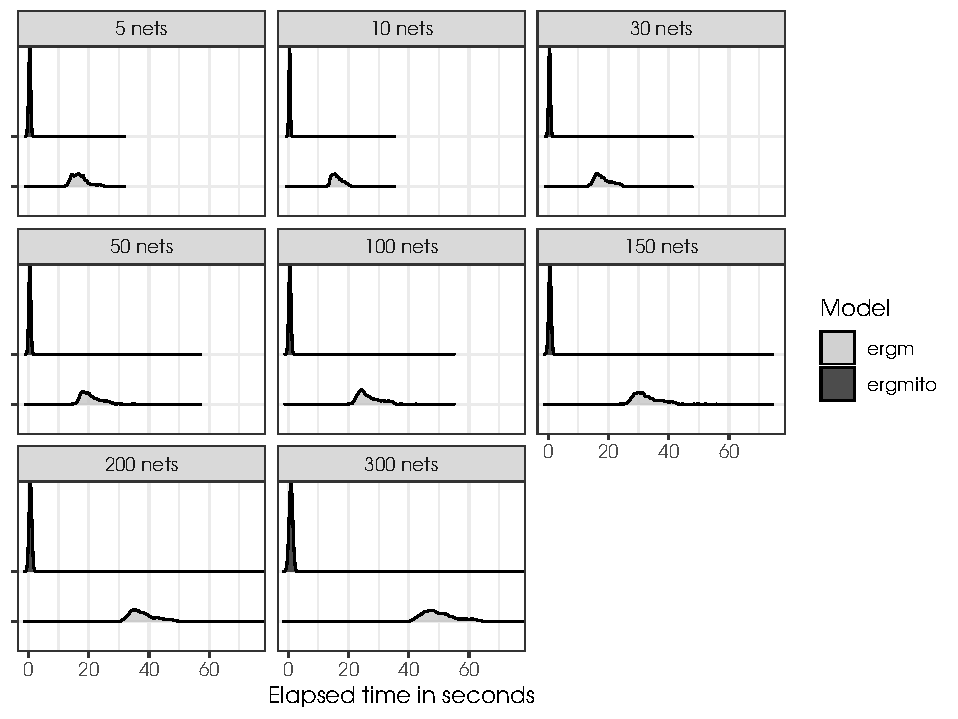
\includegraphics[width=.6\linewidth]{bias-elapsed-02-various-sizes-4-5-ttriad.pdf}
\end{figure}

\vfill\hfill\hyperlink{ergmsims}{\beamergotobutton{more results}}

\end{frame}

% ------------------------------------------------------------------------------
\begin{frame}
\frametitle{Paper 1: Exponential Random Graph Models for Small Networks}

{\bf \large Key takeaways}
\setbeamercolor{conclusions}{bg=usclightgray!60!white, fg=uscdarkgray}
\begin{beamercolorbox}[dp=1ex]{conclusions}
\begin{itemize}[<+->]
\item New extension of ERGMs using exact statistics for small networks
(families, teams, ego-centered, etc.)
\item Performance: Same (un)bias, Lower Type I error rates, (way) faster.
\item Opens the door the new methods.
\end{itemize}
\end{beamercolorbox}

\vfill\pause

{\bf \large Next steps}
\begin{beamercolorbox}[dp=1ex]{conclusions}
\begin{itemize}[<+->]
\item Revisit measurment of goodness-of-fit.
\item Explore extending this method for (very) large networks.
\end{itemize}
\end{beamercolorbox}




\end{frame}


% ------------------------------------------------------------------------------
\section{Paper 2: On the prediction of gene functions using phylogenetic trees}
\cursection

% ------------------------------------------------------------------------------
\begin{frame}
\frametitle{Genes}

How we organize the information about genes (According to the Gene Ontology)

\def\tmpwidth{.9\linewidth}

\begin{table}
\begin{tabular}{*{3}{m{.31\linewidth}<{\centering}}}
\onslide<2->\bf Molecular function & %
\onslide<3->\bf Cellular component & %
\onslide<4->\bf Biological process \\
\onslide<2->\href{http://amigo.geneontology.org/amigo/term/GO:0005215}{Active transport GO:0005215}& %
\onslide<3->\href{http://amigo.geneontology.org/amigo/term/GO:0004016}{Mitochondrian GO:0004016} & %
\onslide<4->\href{http://amigo.geneontology.org/amigo/term/GO:0060047}{Heart contraction GO:0060047} \\
\onslide<2->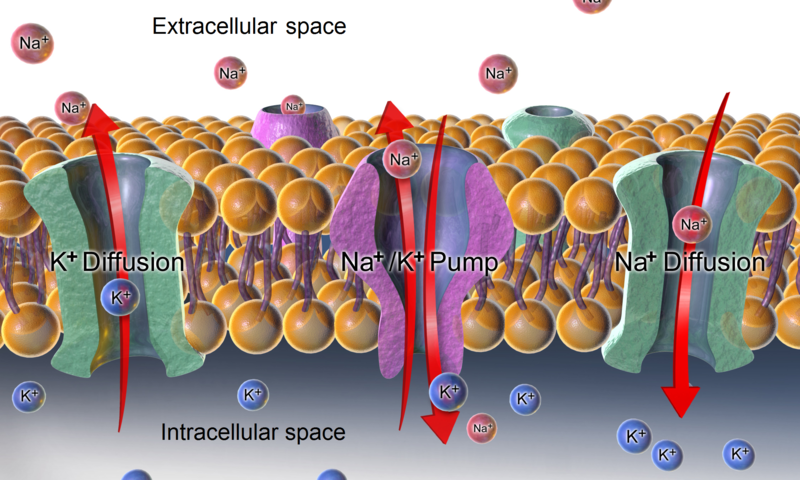
\includegraphics[width=\tmpwidth]{Sodium-potassium_pump_and_diffusion.png} & %
\onslide<3->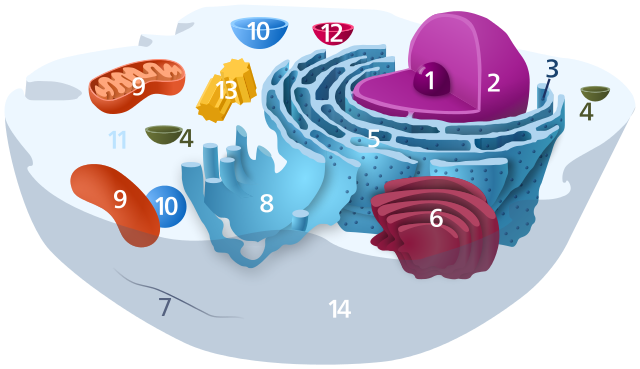
\includegraphics[width=\tmpwidth]{640px-Animal_Cell-svg.png} & % 
\onslide<4->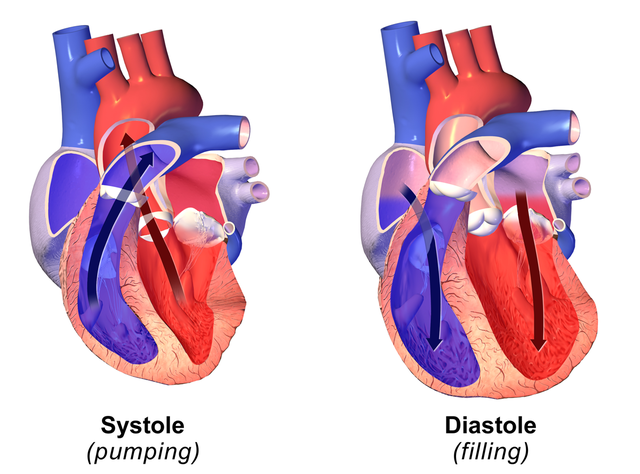
\includegraphics[width=\tmpwidth]{Systolevs_Diastole.png}
\end{tabular}
\end{table}

\end{frame}

% ------------------------------------------------------------------------------
\begin{frame}
\frametitle{Gene Functional Annotations: The Gene Ontology Project}
\begin{itemize}[<+->]
% \item Three domains: Cellular component, molecular function, biological process.
\item Currently, the Gene Ontology Project has: 44,945 validated terms, $\sim$ 6,400,000
annotations on $\sim$ 1,150,000 species.
\item Of all annotations, about $\sim$ 500,000 are on human genes.
\item Knowledge about gene functions can accelerate bio-medical research.
\end{itemize}

\end{frame}

% ------------------------------------------------------------------------------
\begin{frame}
\frametitle{Gene Functional Annotations: The Gene Ontology Project}

Example of GO term

\begin{table}
\footnotesize
\begin{tabular}{lm{.6\linewidth}}
\toprule
\textbf{Accession} & GO:0060047 \\
\textbf{Name} & heart contraction \\
\textbf{Ontology} & biological\_process \\
\textbf{Synonyms} & heart beating, cardiac contraction, hemolymph circulation \\
\textbf{Alternate} & IDs None \\
\textbf{Definition} & The multicellular organismal process in which the heart decreases in volume in a 
characteristic way to propel blood through the body. Source: GOC:dph \\
\bottomrule
\end{tabular}
\caption{Heart Contraction Function. source: \href{http://amigo.geneontology.org/amigo/term/GO:0060047}{amigo.geneontology.org}}
\end{table}\pause

You know what is interesting about this function?

\end{frame}

% ------------------------------------------------------------------------------
\begin{frame}[t]

These four species have a gene with that function... \uncover<2->{and two of %
these are part of the same evolutionary tree!}

\vfill

\def\tmpwidth{.30\linewidth}
\begin{table}
\footnotesize
\begin{tabular}{*{2}{m{\tmpwidth}<\centering}}
\only<1>{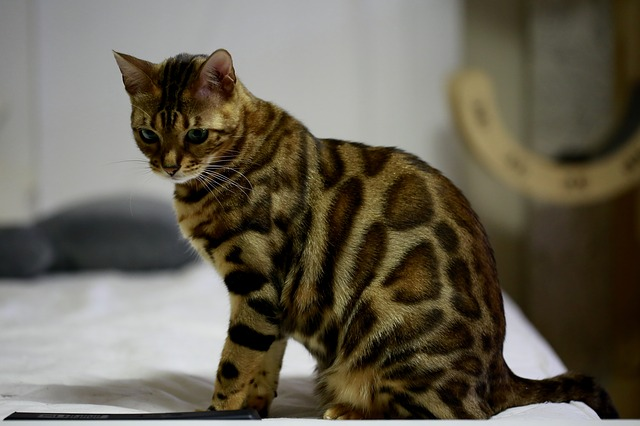
\includegraphics[width=1\linewidth]{cat.jpg}} %
  \only<2>{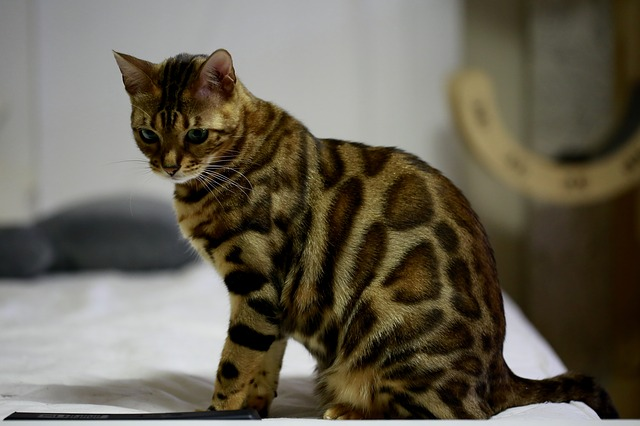
\includegraphics[width=.4\linewidth]{cat.jpg}} \linebreak pthr10037 & %
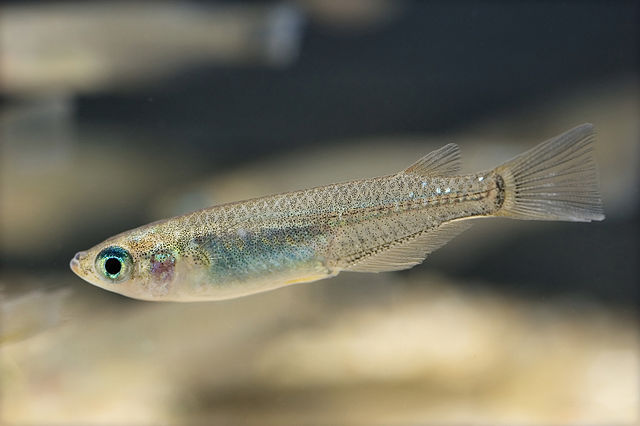
\includegraphics[width=1\linewidth]{Oryzias_latipes.jpg} \linebreak \textbf{pthr11521} \\ %
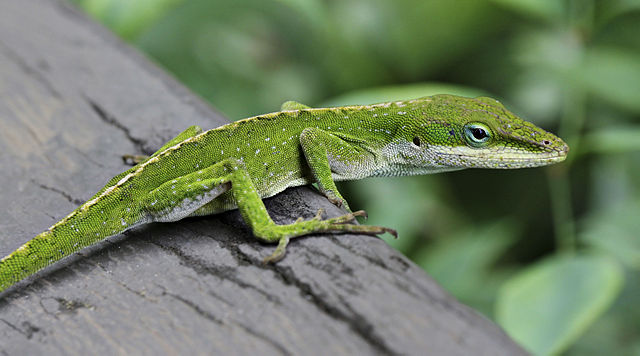
\includegraphics[width=1\linewidth]{Anole_Lizard.jpg} \linebreak \textbf{pthr11521} & %
\only<1>{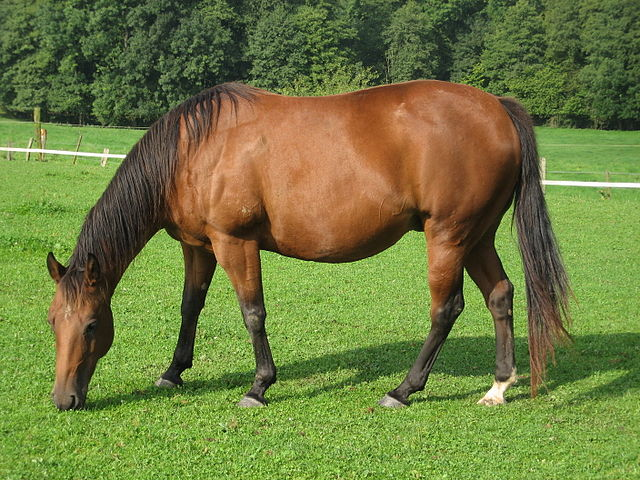
\includegraphics[width=1\linewidth]{horse.jpg}} %
  \only<2>{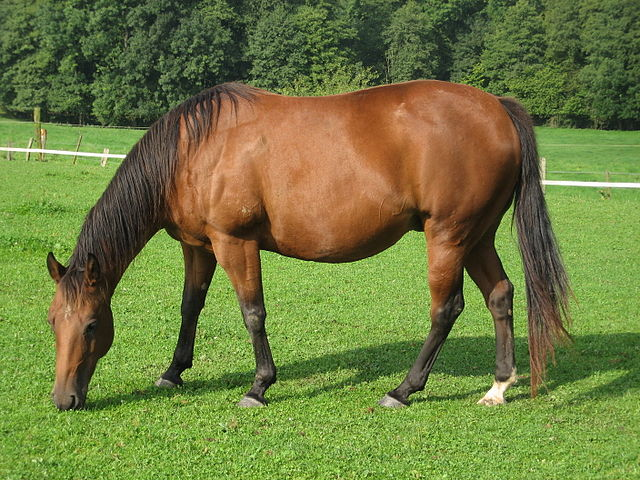
\includegraphics[width=.4\linewidth]{horse.jpg}} \linebreak pthr24356
\end{tabular}
\end{table}
\end{frame}

% ------------------------------------------------------------------------------
\begin{frame}[t]
\frametitle{Phylogenetic Trees}
\begin{minipage}{.4\linewidth}
\pause
\begin{itemize}[<+->]
\item It can be very general: think of the tree of life
\item Nowadays, thanks to gene-sequencing techniques, we are building trees at the
gene level.
\item A single phylogenetic tree can host multiple species
\end{itemize}
\end{minipage}
\hfill
\begin{minipage}{.5\linewidth}
\uncover<5->{
\begin{knitrout}
\definecolor{shadecolor}{rgb}{0.969, 0.969, 0.969}\color{fgcolor}\begin{figure}

{\centering 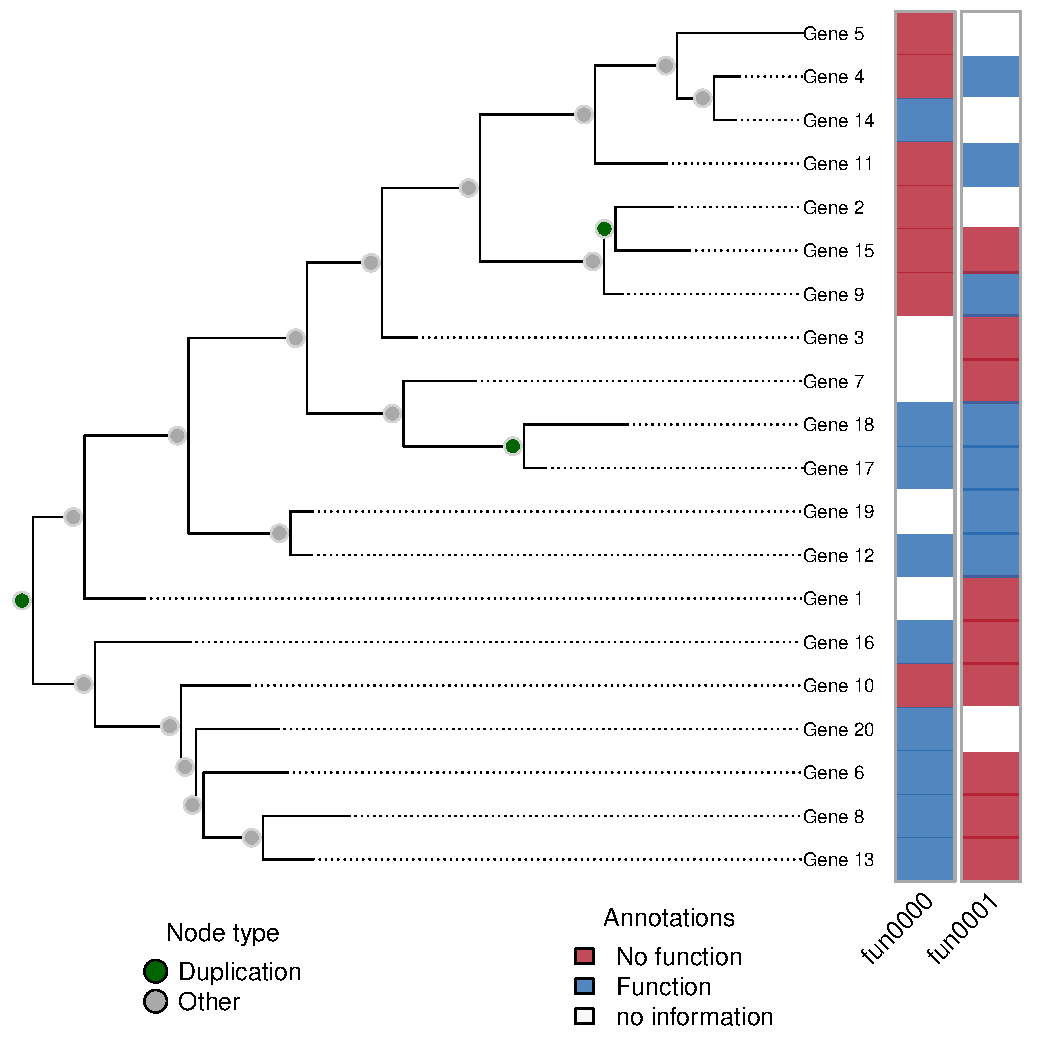
\includegraphics[width=.85\linewidth]{figure/random-tree-1} 

}

\caption[Random annotated phylogenetic tree]{Random annotated phylogenetic tree.}\label{fig:random-tree}
\end{figure}


\end{knitrout}
}
\end{minipage}
\end{frame}


%
\frame{
\centering
\Large
We can use \textcolor{usccardinal}{\bf {\Huge the evolutionary tree}} \\ 
to infer presence/absence of \\
 \textcolor{usccardinal}{{\Huge gene functions (annotations)}!}
}


% ------------------------------------------------------------------------------
\begin{frame}[label=aphylographicalview]
\frametitle{An evolutionary model of gene functions}

\definecolor{rootnode}{RGB}{0,159,211}
\definecolor{innernode}{RGB}{90,159,89}
\definecolor{leafnode}{RGB}{255,107,0}

\begin{minipage}{.48\linewidth}
\begin{itemize}
	\item<2-> \textcolor{rootnode}{Initial (spontaneous) gain of function}.
	\item<3-> \textcolor{innernode}{Loss/gain of offspring depends on: (a) the state of its' parents ({\bf markov process}), and (b) the type of node \hyperlink{duplicationvsspeciation}{\beamergotobutton{more}}}
	\item<4-> \textcolor{leafnode}{We control for human error.}
\end{itemize}
\end{minipage}
%
\begin{minipage}{.50\linewidth}
\begin{figure}
	\footnotesize
	\centering
	\def\svgwidth{.9\linewidth}
	\input{fig/aphylo.pdf_tex}
\end{figure}
\end{minipage}

\vspace{1.5cm}

\uncover<5->{We implemented the model using Felsensteins' pruning algorithm (linear complexity) in the
R package \aphylopkg{} \hyperlink{aphylopkg}{\beamergotobutton{more}}.}

\end{frame}

% ------------------------------------------------------------------------------
\begin{frame}
\frametitle{Prediction with real data}

\begin{table}[ht]
\centering
\scalebox{0.7}{
\begin{tabular}{l*{2}{m{0.1\linewidth}<\centering}*{2}{>{\bf\large}m{0.1\linewidth}<\centering}*{4}{m{0.1\linewidth}<\centering}}
  \toprule
 & (1) & (2) & (3) & (4) & (5) & (6) & (7) & (8) \\ 
  \midrule
$\psi_0$ & 0.00 & 0.00 & 0.23 & 0.25 & 0.00 & 0.00 & 0.21 & 0.25 \\ 
  $\psi_1$ & 0.00 & 0.00 & 0.01 & 0.01 & 0.00 & 0.00 & 0.00 & 0.01 \\ 
  $\mu_{d0}$ & 0.01 & 0.01 & 0.97 & 0.96 & 1.00 & 0.01 & 1.00 & 0.98 \\ 
  $\mu_{d1}$ & 0.01 & 0.02 & 0.52 & 0.58 & 0.25 & 0.02 & 0.51 & 0.58 \\ 
  $\mu_{s0}$ & 0.00 & 0.00 & 0.05 & 0.06 & 0.07 & 0.00 & 0.05 & 0.06 \\ 
  $\mu_{s1}$ & 0.01 & 0.01 & 0.01 & 0.02 & 0.01 & 0.01 & 0.01 & 0.02 \\ 
  $\pi$ & 0.81 & 0.91 & 0.78 & 0.45 & 0.82 & 0.91 & 0.83 & 0.49 \\ 
  Tree count & 88 & 88 & 141 & 141 & 88 & 88 & 141 & 141 \\ 
\midrule   Method & MCMC & MCMC & MCMC & MCMC & MLE & MLE & MLE & MLE \\ 
  Prior & Uniform & Beta & Uniform & Beta & Uniform & Beta & Uniform & Beta \\ 
  Inferred & Yes & Yes & No & No & Yes & Yes & No & No \\ 
  AUC & 1.00 & 1.00 & 0.69 & 0.67 & 0.98 & 1.00 & 0.70 & 0.67 \\ 
  P. Score (obs) & 1.00 & 1.00 & 0.81 & 0.81 & 0.92 & 1.00 & 0.81 & 0.81 \\ 
  P. Score (random) & 0.71 & 0.71 & 0.61 & 0.61 & 0.71 & 0.71 & 0.61 & 0.61 \\ 
   \bottomrule
\end{tabular}
}
\caption{Parameter estimates using different estimation methods, priors, and types of annotations.} 
\end{table}

\end{frame}

% % ------------------------------------------------------------------------------
% \begin{frame}
% \frametitle{Paper 2: Pooled estimation (worth it?)}
% 
% \begin{figure}
% \centering
% 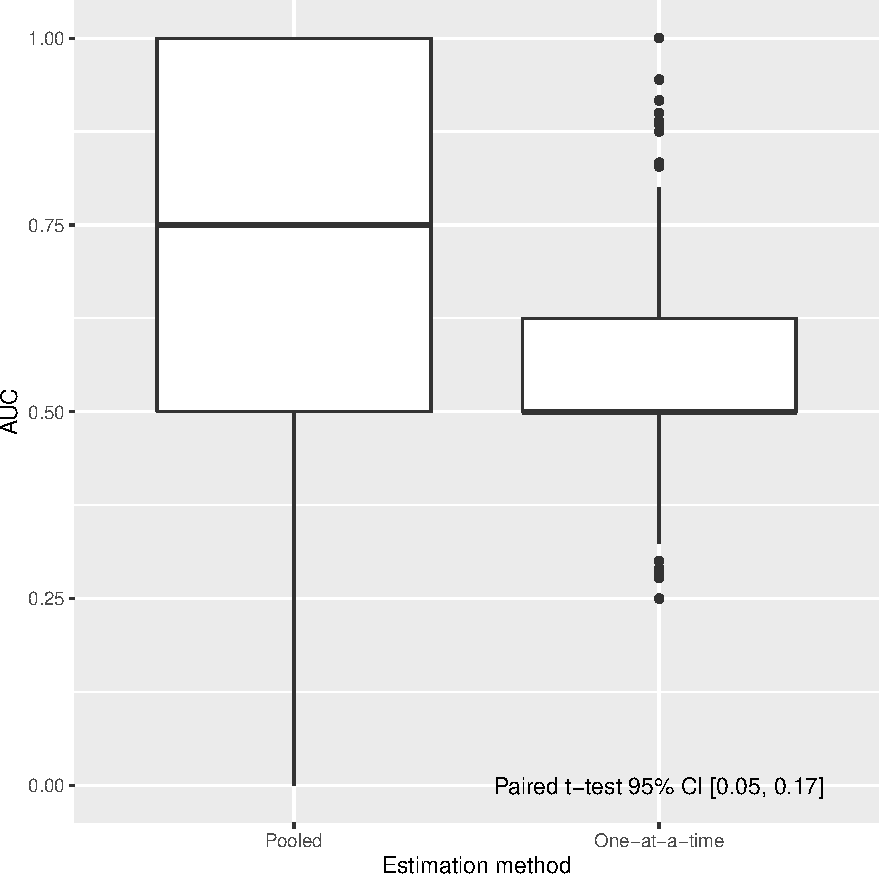
\includegraphics[width=.5\linewidth]{comparing-accuracy-1.pdf}
% \end{figure}
% 
% \end{frame}

% ------------------------------------------------------------------------------
\begin{frame}
\frametitle{Prediction with real data: Leave-one-out}

\begin{figure}
\centering
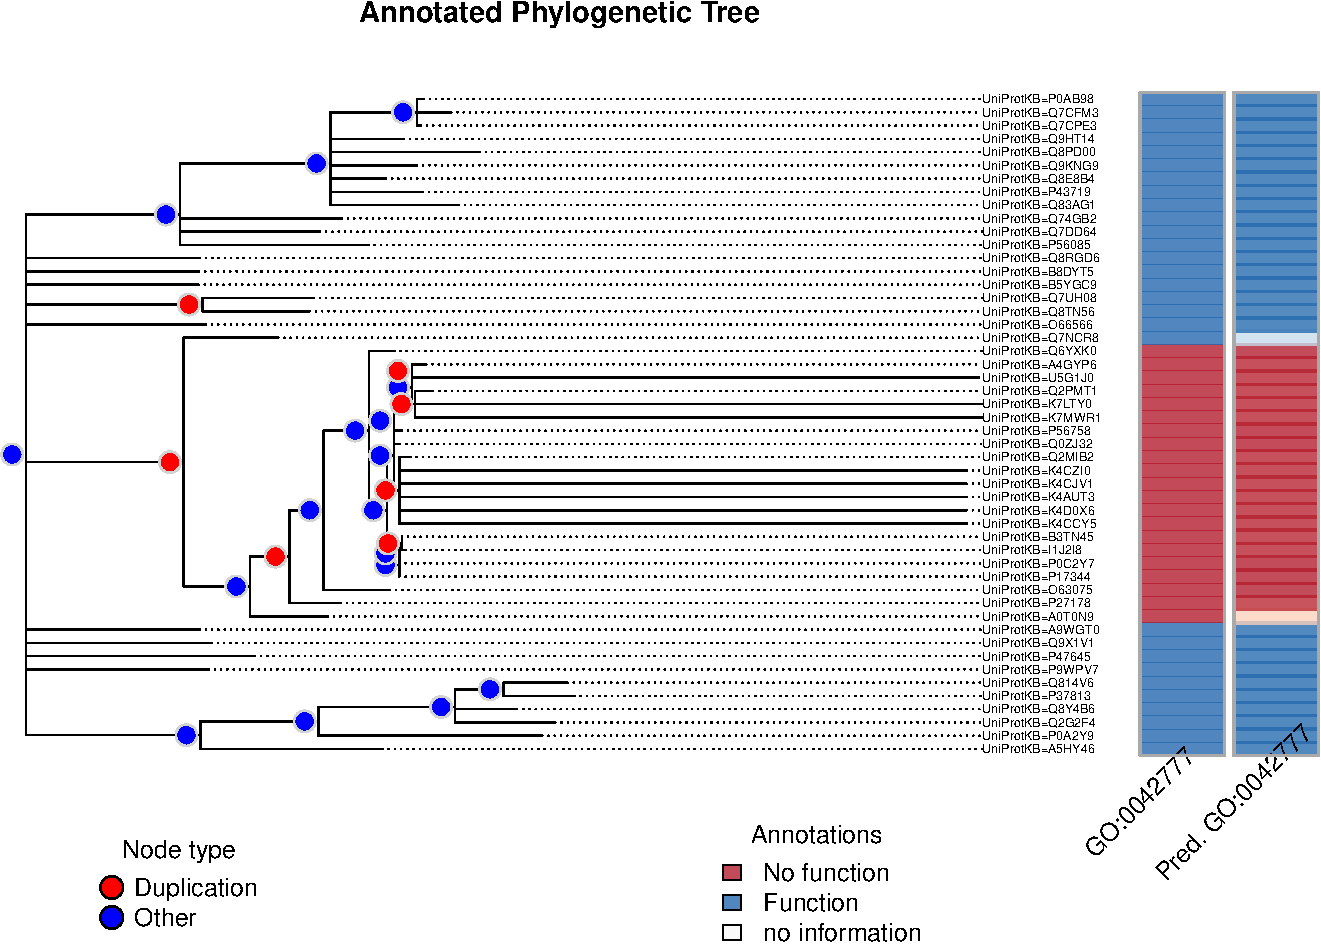
\includegraphics[width=.7\linewidth]{annotations1.pdf}
\end{figure}

\end{frame}

% ------------------------------------------------------------------------------
\begin{frame}
\frametitle{Prediction with real data: Out-of-sample prediction}

\begin{figure}
\centering
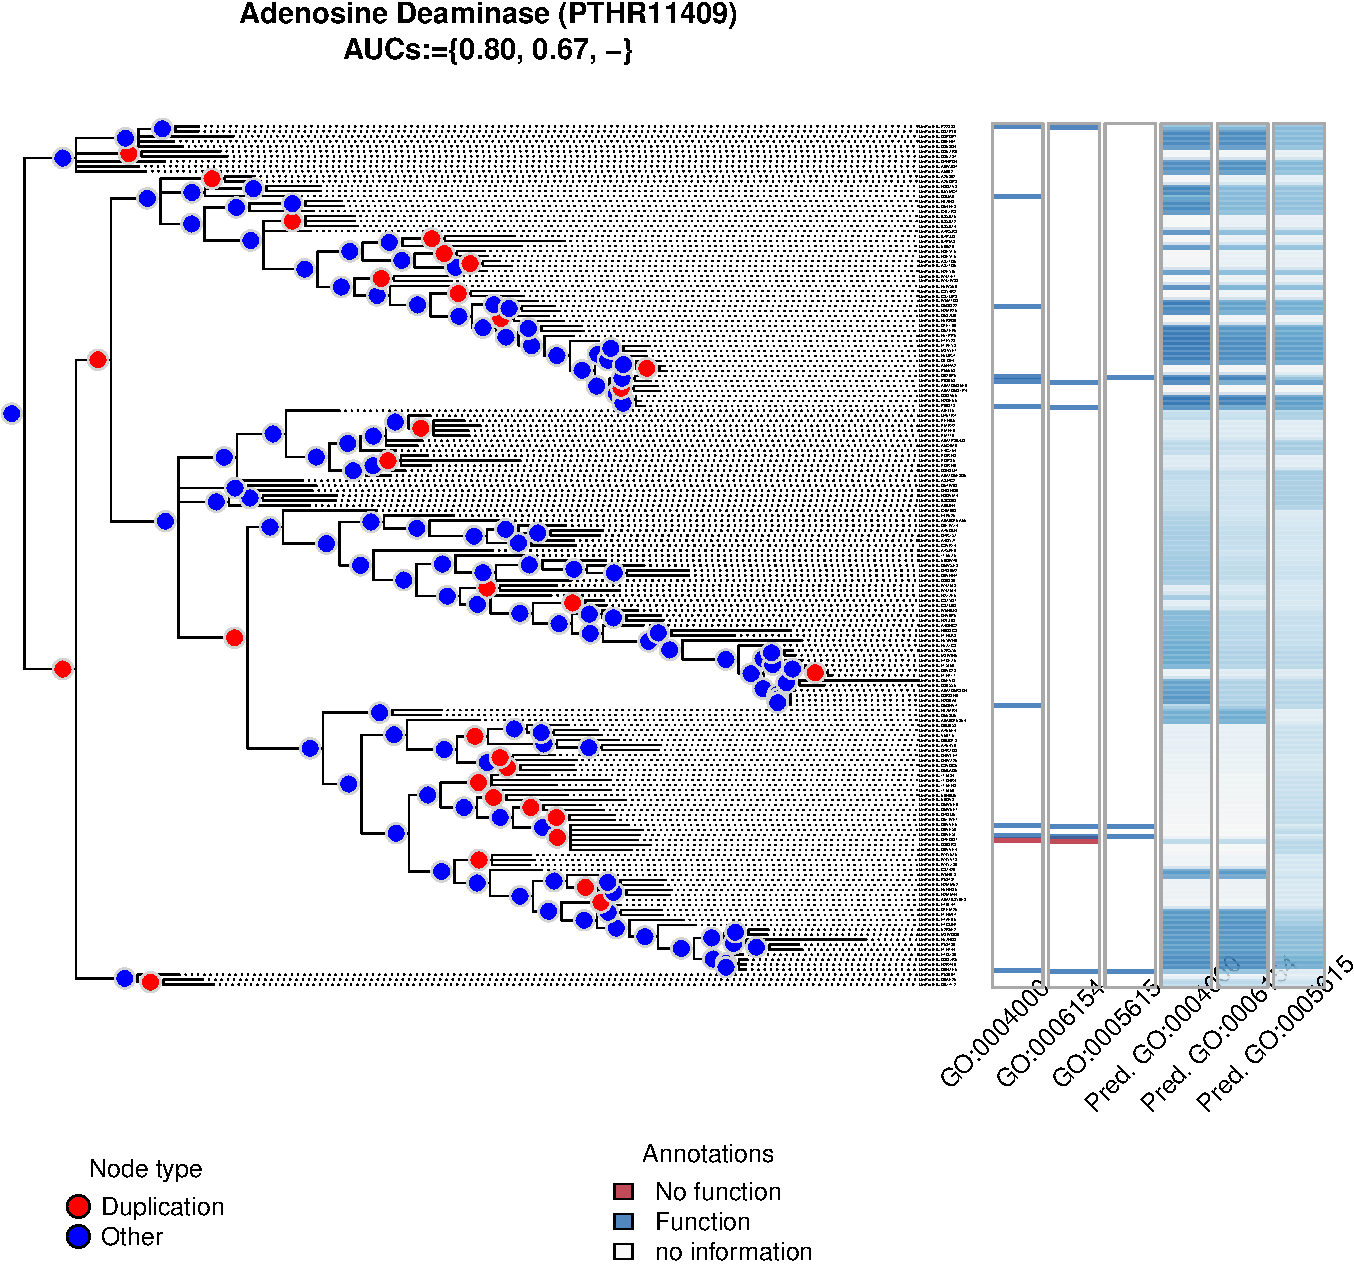
\includegraphics[width=.65\linewidth]{out-of-sample1-1.pdf}
\end{figure}

\end{frame}

% ------------------------------------------------------------------------------
\begin{frame}
\frametitle{Paper 2: On the prediction of gene functions using phylogenetic trees}

{\bf \large Key takeaways}
\setbeamercolor{conclusions}{bg=usclightgray!60!white, fg=uscdarkgray}
\begin{beamercolorbox}[dp=1ex]{conclusions}
\begin{itemize}
\item (Yet another) model for predicting gene functions using phylogenetics.
\item Big difference... computationally scalable.
\item Meaningful biological results.
\item Preliminary accuracy results comparable to state-of-the-art phylo-based models.
\end{itemize}
\end{beamercolorbox}

\vfill\pause

{\bf \large Next steps}
\begin{beamercolorbox}[dp=1ex]{conclusions}
\begin{itemize}
\item Adapt the model to incorporate joint estimation of functions using pseudo-likelihood.
$$
P(a, b, c) \approx P(a,b)P(b,c)P(a,c)
$$
\item Make the model hierarchical when pooling trees: different mutation rates.
\end{itemize}
\end{beamercolorbox}

\end{frame}

% % ------------------------------------------------------------------------------
% \section{Future directions}
% \begin{frame}
% 
% \end{frame}

\begin{frame}
\maketitle
\begin{center}
\scalebox{2}{\textcolor{uscgold}{Thanks!}}
\end{center}
\end{frame}

% ------------------------------------------------------------------------------
\section{Things that are very interesting but I most probably won't have any time to discuss with the attendees}

\begin{frame}
Here are some by-products of my research here at USC

\begin{itemize}
\item The slurmR R package
\item The pruner C++ library
\item The fmcmc R package
\end{itemize}

\end{frame}

\renewcommand{\section}[2]{}%
\appendix
\begin{frame}[allowframebreaks]
\frametitle{References}
\bibliographystyle{apacite}
\bibliography{bibliography.bib}
\end{frame}


% ------------------------------------------------------------------------------
% ------------------------------------------------------------------------------
% ------------------------------------------------------------------------------
% ------------------------------------------------------------------------------
% ------------------------------------------------------------------------------

\begin{frame}[label=ergmterms]

{\bf\color{suffstat} Sufficient statistics} have various forms

\def\fig1width{.45\linewidth}
\begin{figure}[tb]
\centering
\begin{tabular}{m{.2\linewidth}<\centering m{.4\linewidth}<\raggedright}
\toprule Representation & Description  \\ \midrule

\includegraphics[width=\fig1width]{ergm-terms/mutual.pdf} & Mutual Ties (Reciprocity)\linebreak[4]$\sum_{i\neq j}y_{ij}y_{ji}$  \\
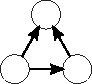
\includegraphics[width=\fig1width]{ergm-terms/ttriad.pdf} & Transitive Triad (Balance)\linebreak[4]$\sum_{i\neq j\neq k}y_{ij}y_{jk}y_{ik}$  \\

\includegraphics[width=\fig1width]{ergm-terms/homophily.pdf} & Homophily\linebreak[4]$\sum_{i\neq j}y_{ij}\mathbf{1}\left(x_i=x_j\right)$ \\
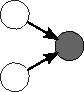
\includegraphics[width=\fig1width]{ergm-terms/nodeicov.pdf} & Covariate Effect for Incoming Ties\linebreak[4]$\sum_{i\neq j}y_{ij}x_j$ \\
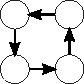
\includegraphics[width=\fig1width]{ergm-terms/fourcycle.pdf} & Four Cycle\linebreak[4]$\sum_{i\neq j \neq k \neq l}y_{ij}y_{jk}y_{kl}y_{li}$  \\
\bottomrule
\end{tabular}
\end{figure}

\vfill\hfill \hyperlink{ergmeq}{\beamerreturnbutton{go back}}
\end{frame}

% ------------------------------------------------------------------------------
\begin{frame}[label=mcmle]
\frametitle{ERGMs: The MC-MLE approach}

One of the most popular methods for estimating ERGMs is the MC-MLE approach (citations here)

This consists on the folling steps

\begin{enumerate}
\item Start from a sensible guess on what should be the population parameters
(usually done using pseudo-MLE esimtation)
\item While the algorithm doesn't converge, do:
  \begin{enumerate}
  \item Simulate a stream of networks with the current state of the parameter,
  $\theta_t$
  \item Using the law of large numbers, approximate the ratio of likelihoods 
  based on the parameter $\theta_t$, this is the objective function
  \item Update the parameter by a Newton-Raphson step
  \item Next iteration
  \end{enumerate}
\end{enumerate}

\vfill\hfill \hyperlink{art}{\beamerreturnbutton{go back}}


\end{frame}

% ------------------------------------------------------------------------------
\begin{frame}[label=ergmitopkg]
\frametitle{The \ergmitopkg{}}

\begin{itemize}
\item Implements estimation of ERGMs using exact statistics for small networks
\item Metaprogramming allows specifying likelihood (and gradient) functions for
joint models
\item Includes tools for simulating, and postestimation checks
\item Getting ready for CRAN!
\end{itemize}

\vfill\hfill \hyperlink{ergmito}{\beamerreturnbutton{go back}}

\end{frame}

% ------------------------------------------------------------------------------
\begin{frame}[label=ergmitodgp]
\frametitle{Paper 1 Simulation Studies}

We performed a simulation study with the following features:

\begin{itemize}[<+->]
\item Draw 20,000 samples of groups of small networks
\item Each group had prescribed: (model parameters, number of networks, sizes of the networks)
\item Each group could have from 5 to 300 small networks
\item We estimated the models using MC-MLE and MLE.
\end{itemize}

\vfill\hfill\hyperlink{ergmitoexample}{\beamerreturnbutton{go back}}

\end{frame}

% ------------------------------------------------------------------------------
\begin{frame}[label=ergmsims,allowframebreaks]
\frametitle{Paper 1 Simulation Studies: Error rate}

\begin{figure}
\centering
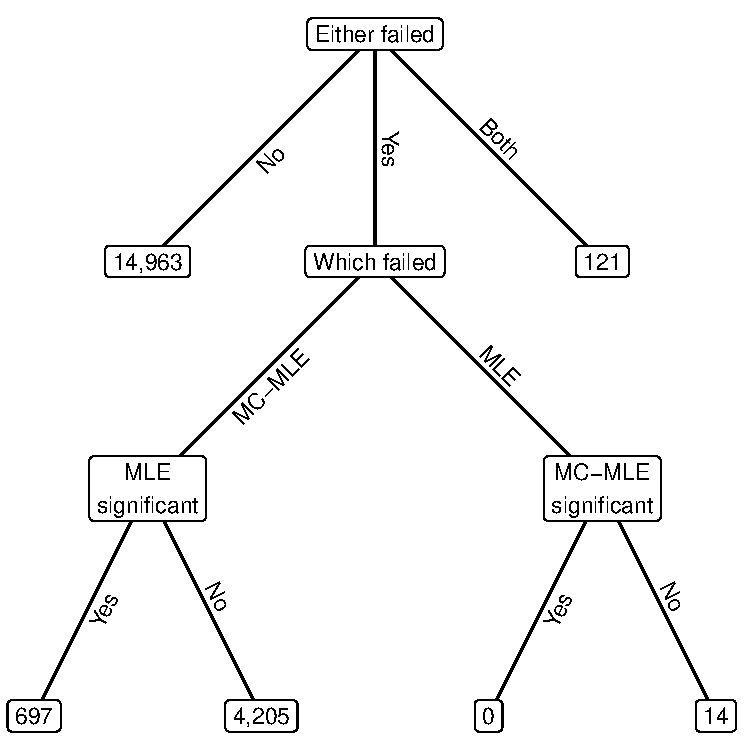
\includegraphics[width=.4\linewidth]{failed-tree.pdf}
\end{figure}

\hyperlink{ergmitoexperiment}{\beamerreturnbutton{go back}}

\end{frame}

\begin{frame}
\frametitle{Paper 1 Simulation Studies: Empirical Bias}

\begin{figure}
\centering
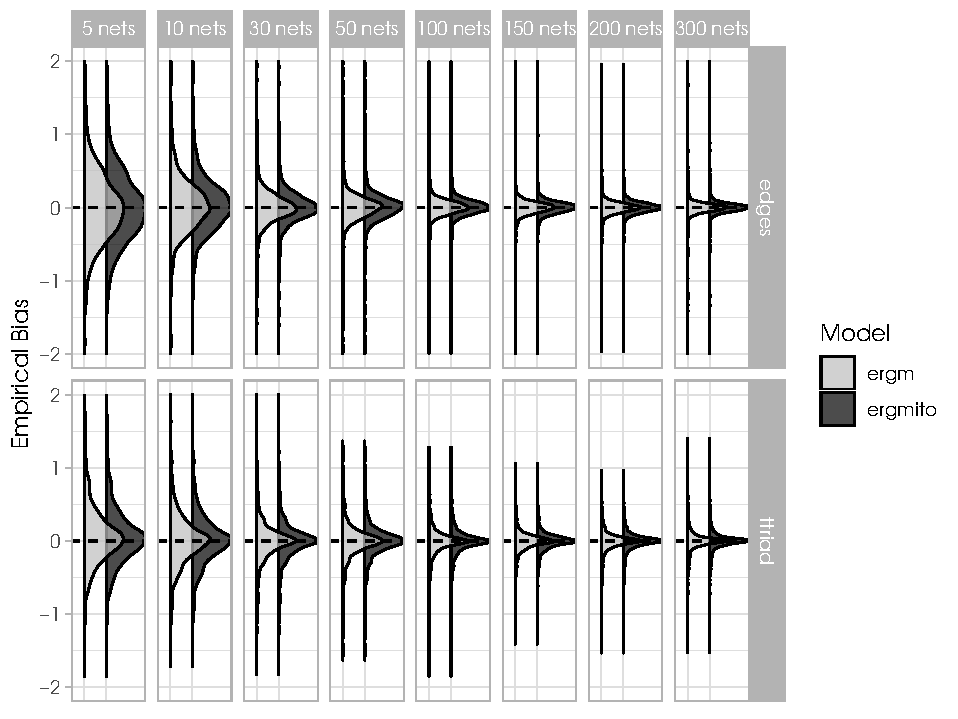
\includegraphics[width=.6\linewidth]{bias-02-various-sizes-4-5-ttriad.pdf}
\end{figure}

\vfill\hfill \hyperlink{ergmitoexperiment}{\beamerreturnbutton{go back}}

\end{frame}

% ------------------------------------------------------------------------------
\begin{frame}[label=aphyloalgorithmicview]
\frametitle{An evolutionary model of gene functions (algorithmic view)}

\scalebox{.7}{

\begin{algorithm}[H]
\SetAlgoLined
\KwData{A phylogenetic tree, $\{\pi, \mu, \psi\}$(Model probabilities)}
\KwResult{An annotated tree}
%\pause
\For{$n \in PostOrder(N)$}{
  $\mbox{\bf\color{usccardinal}Nodes gain/loss function depending on their parent}$\;%\pause
  \Switch{class of $n$}{
    \uCase{root node}{
      Gain function with probability $\pi$\;
    }%\pause
    \uCase{interior node} {%\pause
      \lIf{Parent has the function}{Keep it with prob. $(1-\mu_1)$}%\pause
      \lElse{Gain it with prob. $\mu_0$}%\pause
    }
  }%\pause
  $\mbox{\bf\color{usccardinal}Finally, we allow for mislabeling}$\;%\pause
  \uIf{$n$ is leaf}{%\pause
    \lIf{has the function}{Mislabel with prob. $\psi_1$}%\pause
    \lElse{Mislabel with prob. $\psi_0$}%\pause
  }
}
\end{algorithm}
}

\vfill\hfill \hyperlink{aphylographicalviewcont}{\beamergotobutton{go back}}


\end{frame}

% ------------------------------------------------------------------------------
\begin{frame}[label = duplicationvsspeciation]
\frametitle{Speciation}
\begin{figure}
\centering
\def\svgwidth{.8\linewidth}
\tiny
% Source 
\input{fig/Drosophila_speciation_experiment.pdf_tex}
\caption{\citeA{Dodd1989}: After one year of isolation, flies showed a significant level or assortativity in mating (\href{https://commons.wikimedia.org/wiki/File:Drosophila_speciation_experiment.svg}{wikimedia})}
\end{figure}

\vfill\hfill \hyperlink{aphylographicalview}{\beamerreturnbutton{go back}}

\end{frame}

\begin{frame}
\frametitle{Duplication}
\begin{figure}
\centering
\def\svgwidth{.6\linewidth}
\tiny
% Source : https://en.wikipedia.org/wiki/File:Evolution_fate_duplicate_genes_-_vector.svg
\input{fig/Evolution_fate_duplicate_genes_-_vector.pdf_tex}
\caption{A key part of molecular innovation, gene duplication provides opportunity for new functions to emerge (\href{https://en.wikipedia.org/wiki/File:Evolution_fate_duplicate_genes_-_vector.svg}{wikimedia})}
\end{figure}

\vfill\hfill \hyperlink{aphylographicalviewcont}{\beamerreturnbutton{go back}}

\end{frame}

% ------------------------------------------------------------------------------
\begin{frame}[label=aphylopkg]
\frametitle{The \aphylopkg{}}

\begin{itemize}
\item Pruning algorithm implemeted in C++ using the \texttt{pruner} template library (implemeted in this project).
\item The estimation is done using either Maximum Likelihood, Maximum A Posteriory, or MCMC.
\item The MCMC estimation is done via the \texttt{fmcmc} R package using adaptive MCMC
(also implemeted as part of this project)
\end{itemize}

\vfill\hfill \hyperlink{aphylographicalviewcont}{\beamerreturnbutton{go back}}
\end{frame}

\end{document}

